There are three steps as follows.
\begin{enumerate}
  \item \textbf{Collecting} all \emph{simple transition paths}.
  Every \emph{simple transition paths}, $\tpath \in \paths(\absG(c))$ 
  contains only the edges of atomic assignment or guard transitions without interleaving other paths.
  Each of them corresponds to a path in the flatten program in Definition~4.1 in \cite{GulwaniJK09}.
  \item \textbf{Rewriting} the program $c$ by rearranging all \emph{simple transition paths} as the syntax in \cite{GulwaniJK09} and preserves the same semantics.
  \item \textbf{Refining} the program and computing the 
  refined program, $\rprog$ by Algorithm~1 in paper~\cite{GulwaniJK09}.
  This step invokes the algorithm REFINE from paper~\cite{GulwaniJK09} and compute the 
  refined program $\rprog$ for a program $c$ given the rewritten program as input.
\end{enumerate}

\subsection{The Simple Transition Path}
We first collect the loop headers $\loopl(c) \subseteq \lvar(c)$ from a program $c$, which is the set of all program points corresponding to the loop headers in program $c$.
\begin{defn}[Loop Headers ($\loopl : \cdom \to \mathcal{P}(\ldom)$)]
  \label{def:loopl}
  \[
  \loopl(c) \triangleq 
  \left\{
    \begin{array}{ll}
      \{\}  & {c} = \clabel{\assign x e}^{l} \\
      \loopl({c_1}) \cup \loopl({{c_2}})  & {c} = {c_1};{c_2} \\
      \loopl(c_t) \cup \loopl({{c_f}})   & {c} =\eif(\clabel{\bexpr}^{l}, c_t, c_f) \\
  \loopl(c_w) \cup \{l\}, &  {c}   = \ewhile \clabel{\bexpr}^{l} \edo (c_w)
  \end{array}
\right.
\]
  \end{defn}
% \begin{defn}[Loop Path]
%   \label{def:looppath}
% A simple transition path
% $\tpath \in \paths(\absG(c))$ for the program $c$, is a path on its abstract transition graph $\absG(c) = (\absV(c), \absE(c))$ with 
% \begin{itemize}
% \item a vertices sequence $(l_0, \ldots, l_n)$, where $l_i \in \absV(c)$ for every $i = 0, \ldots, n$ and
% %
% \item an edge sequence $(e_1, \ldots, e_n)$, where $e_i = (l_{i - 1}, dc_i, l_{i}) \in \absE(c)$ for every $i = 1, \ldots, n$,
% \end{itemize}
% %
% satisfying:
% \begin{itemize}
%   \item $l_i \neq l_j$ for every $i = 0, \ldots, n$ and $j = 0, \ldots, {n - 1}$,
%   \item $l_0$ is either the program point of a loop header or the program entrance ($l_0 = 0$),
%   i.e., $l_0 \in \loopl(c) \cup \{ 0 \}$
%   \item and $l_n$ is either the program point of a loop header or the program exit ($l_n = \lex$),
%   i.e., $l_0 \in \loopl(c) \cup \{ \lex \}$.
% \end{itemize}
% \end{defn}

\begin{defn}[Simple Tansition Path]
  \label{def:tpath}
A \emph{simple transition path}
$\tpath \in \paths(\absG(c))$ for the program $c$, is either a simple cyclic path, which has the same start- and end-point
or a simple path has either different while loop headers, the program entrance or exit as its start- and end-point
without visiting any loop header inside the path.
\\
Specifically, a path $l_0 \xrightarrow{dc_0} l_1 \xrightarrow{dc_1} \ldots l_n \in \paths(\absG(c))$ with the
vertices sequence $(l_0, \ldots, l_n)$, where $l_i \in \absV(c)$ for every $i = 0, \ldots, n$ and
%
the edge sequence $(e_1, \ldots, e_n)$, where $e_i = (l_{i - 1}, dc_i, l_{i}) \in \absE(c)$ for every $i = 1, \ldots, n$,
%
is a \emph{simple transition path} if and only if it satisfies,
\begin{itemize}
  \item $l_i \neq l_j$ for every $i = 0, \ldots, n$ and $j = 0, \ldots, {n - 1}$,
  \item $l_0$ is either the program point of a loop header or the program entrance ($l_0 = 0$),
  i.e., $l_0 \in \loopl(c) \cup \{ 0 \}$
  \item and $l_n$ is either the program point of a loop header or the program exit ($l_n = \lex$),
  i.e., $l_0 \in \loopl(c) \cup \{ \lex \}$,
  \item and $l_i \notin \loopl(c) \cup \{ 0, \lex \}$ for every $i = 1, \ldots, n-1$.
\end{itemize}
\end{defn}


\paragraph{Example.}
% \todo{The walk through example}
For example in Figure~\ref{fig:relatedNestedWhileOdd-overview}(b), the $1 \to 2 \to 8 \to 1$ is a \emph{simple transition path}.
However, $1 \to 2 \to 3 \to 4 \to 5 \to 4 \to 6 \to 7 \to 1$ is not a \emph{simple transition path} because it is not simple.
Also, $1 \to 2 \to 3 \to 4 \to 6 \to 7 \to 1$ is not a \emph{simple transition path} because it visits a loop header $4$ inside the path. $1 \to 2 \to 3$ isn't either because its end-point isn't a loop header.
In Figure~\ref{fig:threeWhile-overview}(b), $1 \to 2 \to 3 \to 4 \to 5 \to 6$ is not a \emph{simple transition path} on $\absG(\kw{threeNestedWhile}(n, m, N))$ because it visits a loop header $3$ inside the path.

\subsection{Program Rewrite}
\paragraph{Syntax.}

\paragraph{Rewrite Algorithm.}
\begin{algorithm}
  \caption{Program Rewriting $\kw{Rewrite}$}
  \label{alg:alg-refine_rewrite}
  \begin{algorithmic}[1]
    \REQUIRE program $c$ and all \emph{simple transition path}s, $\tpath_1, \ldots, \tpath_n \in \paths(\absG(c))$.
    % \STATE collects all $c$'s \emph{simple transition path}s from $\absG(c)$, $\tpath_1, \ldots, \tpath_n \in \paths(\absG(c))$.
    \STATE \textbf{init}: candidate set $W = \{c_1, \ldots, c_n\}$, where $c_i = \tpath_i$ and $i = 1, \ldots, n$
    \STATE \textbf{while} $W.size()> 1$:
    \STATE \quad 
    for all $c_i \in W \land c_i.start = c_j.start \land c_i.end = c_j.end, i, j = 1, \ldots, n$.
    \\ \quad create $c' = \rpchoose{c_1, \ldots, c_m}$, \qquad  $W.add(c')$ \qquad $W.remove(c_1, \ldots, c_m)$
    \STATE
    \quad for all $c_i \in W \land c.start = c.end \land c.start \in \loopl(c)$
    \\ \quad create $c' = \rprepeat(c)$, \qquad $W.add(c')$, \qquad $W.remove(c)$
    \STATE \quad for all $c_1, c_2 \in W \land c_1.end = c_2.start$
    \\
    \quad create $c' = c_1; c_2$, \quad $W.add(c')$ \qquad $W.remove(c_1, c_2)$
    % \STATE \textbf{Endwhile}
    \RETURN $W[0]$.
  \end{algorithmic}
  \end{algorithm}
%
Algorithm~\ref{alg:alg-refine_rewrite} transformation the syntax of program following~\cite{GulwaniJK09} and preserving the semantics.
We first use simple depth first search strategy collects all the \emph{simple transition path}s satisfying the Definition~\ref{def:tpath}. It guarantees that every $\tpath$ is equivalent to a path $\rho$ in Definition~4.1 of \cite{GulwaniJK09}.
Then
in Line-2, we initialize each candidate $c_i$ with a \emph{simple transition path} $\tpath_i$. New candidates generated in Line-4, 5 and 6 correspond to the if,
while and sequence statement in paper~\cite{GulwaniJK09} respectively.
\begin{itemize}
  \item
  Line-4: for all the candidates $c_1, \ldots, c_m$ having the same starting and ending vertices, rewrite them into if statement as~\cite{GulwaniJK09}.
  \item
  Line-5: for every candidate $c'$, if it starts and ends with the same vertex, rewrite it into while loop statement as~\cite{GulwaniJK09}.
  \item
  Line-6: for every two candidates $c_1, c_2$, if $c_1$ ends with the same vertex as $c_2$'s starting label, rewrite them into sequence statement as~\cite{GulwaniJK09}.
\end{itemize}
% \todo{soundness of the program write}
\subsection{Program Refinement}
% We implement the algorithm REFINE from paper~\cite{GulwaniJK09} and compute the 
% refined program $\rprog$ for a rewritten program $c$.

\paragraph{Contextualization}

$cxlE$ is a set of edges between two simple transition paths of program $c$. There is an edge from $\tpath_1$ to $\tpath_2$
if and only if $\tpath_2$ can execute right after execution of $\tpath_1$.
% We adopt the contextualization method from paper~\cite{ZulegerGSV11} Definition~10 and build the edge.

\paragraph{Path Interleaving Refinement}
\begin{algorithm}
  \caption{
  {Interleaving Refinement}
  \label{alg:prog-refine}
  }
  \begin{algorithmic}[1]
  \REQUIRE $\absG(c)$, the contextualization $cxlG(c)$.
  % the target while loop with label $l$.
  \STATE  \textbf{Init} 
  % \\
  $R_l = \{\}$ initial set for each loop with header at program point $l$, (i.e., set of the transition sequences from interleaving-refinement) .
  % \STATE \todo{Define algorithm $\kw{dfs(w, I_{l}, FS)}$}
  \STATE Define algorithm \highlight{$\kw{dfs(w, I_0, Q)}$:}
  \STATE \quad {$\kw{I = Q.top}$:}
  \STATE \quad \textbf{For} each simple transition path $\tpath'$ that can execute right after $\tpath$,
  $(\tpath, \tpath') \in cxlE(c)$ and $\tpath \neq \tpath'$;
  \\
  % \\
  \STATE \quad \quad $\kw{w' = w.append(\tpath')}$
  \\
  \quad \quad \highlight{Compute Invariant $\kw{I' = API(\tpath', I)}$}
  \STATE  \quad \quad Compute the exiting condition of $\tpath'$ (/ or Invariant by  API) $I'$ and the 
  post condition (or final state) of executing $\tpath'$, $FS'$.
  \STATE \quad \quad \textbf{If} \highlight{$\kw{I' \in Q}$}
  \STATE \quad \quad \textbf{then}
  % let $i$ be the index such that 
  Let $w = [\tpath_1, \ldots; \tpath_n]$, $Q = [I_1, \ldots, I_n]$, and $i$ be the index such that $I_i = I'$
  \\ \quad \quad \quad \quad \quad
  $\kw{R_l.append(\tpath_1; \ldots; \tpath_{i - 1}; (\tpath_i; \ldots; \tpath')^*)}$
  % \STATE \quad \quad \todo{\textbf{else} $\kw{dfs(w', I_l, FS')}$}
  \STATE \quad \quad  \highlight{\textbf{else If} 
  $\kw{I' \neq \bot}$ \textbf{then} ${\kw{dfs(w', I_0, Q.push(I'))}}$}
    \STATE \textbf{For} each loop program $c_{l}$ with header at program point $l$, 
    \STATE \quad \highlight{Compute Invariant $\kw{I_0 = API(c_{l}, \etrue)}$}
    \STATE \quad computing $\kw{dfs([], I_0, [I_0] )}$
  \RETURN $R_l$ for every while loop with its header at $l$.
  \end{algorithmic}
  \end{algorithm}



The interleaving refinement method compute the execution order of each simple transition paths explicitly.

For example, two simple transition paths $\tpath_1 = (1 \to 2 \to 3 \to 4)$ and 
$\tpath_4 = (1 \to 2 \to 8 \to 1)$ in the same loop Figure~\ref{fig:relatedNestedWhileOdd-overview}(b) have two possible execution orders:
either $\tpath_1$ executes immediately after the execution of $\tpath_4$, or vice verse.
% and compute the 

Then we construct the refined program by explicating the execution orders of simple transition paths.
% refined program $\rprog$ for a rewritten program $c$.
Simple transition paths can iterate on themselves, so an execution order could
contain iterations of simple transition paths, and sequence of iterations.

For example, the simple transition path $\tpath_3 = (4 \to 5 \to 4)$
the loop $L_4$ in Figure~\ref{fig:relatedNestedWhileOdd-overview}(b) has only one possible execution order,
which is the iteration on itself, $\rprepeat(\tpath_3)$.
Each loop in a refined program contains several execution orders over its original simple transition paths.
For example, the loop $L_1$ in Figure~\ref{fig:relatedNestedWhileOdd-overview}(b)
has two execution orders. In the first one,
$\rprepeat(\tpath_4; \tpath_1; 4:\rprepeat(\tpath_3); \tpath_2)$ 
$\tpath_1$ will execute right after the execution of $\tpath_4$.
Then following the execution of $\tpath_1$, loop $L_4$ finishes full iterations and followed by the execution of $\tpath_2$.
In the second execution order,
$\rprepeat(\tpath_1; 4:\rprepeat(\tpath_3); \tpath_2; \tpath_4)$,
$\tpath_4$ is executed after the execution of $\tpath_1; 4:\rprepeat(\tpath_3); \tpath_2$.
Iteration of one execution order is equivalent to one possible full iterations of the original loop program.
So the reconstructed loop for $L_1$ is 
\[
\rpchoose{ 
 \begin{array}{l}
 1: \rprepeat(\tpath_1; 4:\rprepeat(\tpath_3); \tpath_2; \tpath_4), \\
 1: \rprepeat(\tpath_4; \tpath_1; 4:\rprepeat(\tpath_3); \tpath_2) 
 \end{array}
 }.
\]

\paragraph{Running Example.}
For the walk-through an example in Figure~\ref{fig:relatedNestedWhileOdd-overview}(b),
We first collect all its simple transition paths from $\absG(\kw{relatedNestedWhileOdd}(n, m))$ as
$\tpath_0 = (0 \to 1)$,
$\tpath_1 = (1 \to 2 \to 3 \to 4)$,
$\tpath_2 = (4 \to 6 \to 7 \to 1)$,
$\tpath_3 = (4 \to 5 \to 4)$, $\tpath_4 = (1 \to 2 \to 8 \to 1)$, and $\tpath_5 = (1 \to \lex)$.
Using these simple transition paths, we first rewrite this program by Algorithm~\ref{alg:alg-refine_rewrite} and get the rewritten program
%  corresponding to the syntax in~\cite{GulwaniJK09} as
$ \tpath_0 ; \rpchoose{ 1: \rprepeat(\tpath_1; 4:\rprepeat(\tpath_3); \tpath_2), 
1: \rprepeat(\tpath_4) }; \tpath_5$.
Then we construct the refined program as,
\[
 \tpath_0 ; \rpchoose{ 
 \begin{array}{l}
 1: \rprepeat(\tpath_1; 4:\rprepeat(\tpath_3); \tpath_2; \tpath_4), \\
 1: \rprepeat(\tpath_4; \tpath_1; 4:\rprepeat(\tpath_3); \tpath_2) 
 \end{array}
 }; \tpath_5.
\]

\paragraph{Example II.}
We present again the motivating example program from Figure~\ref{fig:whileTwoCounters-overview}(a)
below in Figure~\ref{fig:whileTwoCounters-refine}(a)
%   another example from the .Net base-class library 
to show the necessity of the \emph{path refinement}. 
%   It 
It has a two paths loop
with different \emph{reachability-bound}s on the locations of different paths.
%
%
{ 
\begin{figure}
\centering
%
\begin{subfigure}{.35\textwidth}
    $
    \begin{array}{l}
      \kw{twoPathsWhile}(n, m) \triangleq \\
    \clabel{ \assign{i}{n} }^{0} ;
    \clabel{ \assign{j}{0} }^{1} ; \\
    L_2:    \ewhile ~ \clabel{i > 0}^{2} ~ \edo ~ \\
        \qquad \big(
          \eif(\clabel{j < m}^{3}, \\
          \qquad \ethen  \clabel{\assign{j}{j + 1}}^{4}; \\
          \qquad \qquad \clabel{\assign{i}{i - 1}}^{5},\\
          \qquad \eelse \clabel{\assign{j}{0}}^{6});
          \big)
        \end{array}
        $
\caption{}
\end{subfigure}
\begin{subfigure}{.6\textwidth}
\begin{centering}
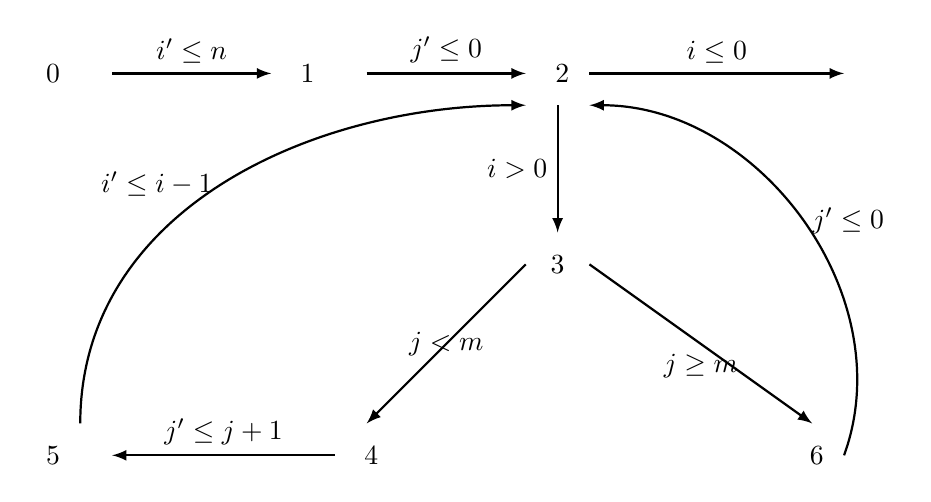
\begin{tikzpicture}[scale=\textwidth/15cm,samples=200]
\draw[] (-8, 10) circle (0pt) node{{ $0$}};
\draw[] (-4, 10) circle (0pt) node{{ $1$}};
\draw[] (0, 10) circle (0pt) node{{ $2$}};
\draw[] (0, 7) circle (0pt) node{{$3$}};
\draw[] (-3, 4) circle (0pt) node{{ $4$}};
\draw[] (-8, 4) circle (0pt) node{{ $5$}};
\draw[] (4, 4) circle (0pt) node{{ $6$}};
\draw[] (5, 10) circle (0pt) node {\textbf{$\lex$}};
%
\draw[ thick, -latex] (-7, 10)  -- node [above] {$i' \leq n$}(-4.5, 10);
\draw[ thick, -latex] (-3, 10)  -- node [above] {$j' \leq 0$}(-0.5, 10);
\draw[ thick, -latex] (0, 9.5)  -- node [left] {$i > 0$} (0, 7.5) ;
\draw[ thick, -latex] (0.5, 7)  -- node [below] {$ j \geq m $}  (4, 4.5);
\draw[ thick, -latex] (-7.5, 4.5)  to  [out=90,in=180]  node [left] {$i' \leq i - 1$ }(-0.5, 9.5);
\draw[ thick, -latex] (4.5, 4)  to  [out=70,in=0]   node [right] {$j' \leq 0 $}(0.5, 9.5);
\draw[ thick, -latex]  (-0.5, 7) -- node  {$j < m$}  (-3, 4.5) ;
\draw[ thick, -latex]  (-3.5, 4) -- node [above] {$j' \leq j + 1$}  (-7, 4) ;
\draw[ thick, -latex] (0.5, 10)  -- node [above] {$i \leq 0$}  (4.5, 10);
\end{tikzpicture}
    \caption{}
\end{centering}
\end{subfigure}
{\small
\begin{subfigure}{.8\textwidth}
\begin{centering}
    $\tpath_0 = 0 \to 1 \to 2$,
    $\tpath_2 = 2 \to 3 \to 6 \to 2$, \\
    $\tpath_1 = 2 \to 3 \to 4 \to 5 \to 2$,
    $\tpath_3 = 2 \to \lex$\footnotemark
    \caption{}
\end{centering}
\end{subfigure}
}
{
\begin{subfigure}{.8\textwidth}
\begin{centering}
$
\tpath_0; 
\rpchoose{ 2: \tpath_1, 2: \tpath_2 }; \tpath_3.
$
\caption{}
\end{centering}
\end{subfigure}
}
\begin{subfigure}{.8\textwidth}
  \begin{centering}
  $
  \tpath_0 ; 
  \rpchoose{2: \rprepeat(\rprepeat(\tpath_1); \tpath_2), 
  2: \rprepeat(\tpath_1)}; \tpath_3.
  $
  \caption{}
\end{centering}
  \end{subfigure}
\caption{
(a) The two paths loop example.
(b) The abstract transition graph for $\kw{twoPathsWhile}(n, m)$.
(c) The simple transition paths.
(d) The rewrote program.
(e) The refined program.}
    \label{fig:whileTwoCounters-refine}
\end{figure}
}

%
%  To know the bounds for locations on different branches of a loop, 
%  it is necessary to know the alternating patterns of the two paths.
Over its abstract transition graph in Figure~\ref{fig:whileTwoCounters-refine}(b), we first collect all its simple transition path as in Figure~\ref{fig:whileTwoCounters-refine-overview}(c).
Then we transform the multiple-path loop by computing the interleaving between paths explicitly and
generates a refined program $\rprog$ as the bottom part of Figure~\ref{fig:whileTwoCounters-refine}.

We first compute that $\tpath_1$ can iterate on itself, so there is one possible execution sub-order,
$\rprepeat(\tpath_1)$.
We recursively compute that after $\tpath_1$ done with the iteration on itself,
either the iteration of the original loop is finished
or $\tpath_2$ can execute right after.
For the first case, we compute a complete execution order $\rprepeat(\tpath_1)$.
In the second case, we again have a possible execution sub-order, $\rprepeat(\tpath_1); \tpath_2$.
After execution of $\tpath_2$, we compute that $\tpath_1$ iterates on itself again
and goes back to the same execution sub-order. 
The refinement algorithm finds this repetition and generate a complete execution order
$\rprepeat(\rprepeat(\tpath_1); \tpath_2)$.
Then the algorithm finish the refinement process since there is no more sub-orders. 
%  In the first one, $\tpath_2$ will be executed after all the iterations of $\tpath_1$ are done, and in the second one,
%  the entire loop is done after $\tpath_1$ finishes the iteration.
The refined program then is constructed below as in Figure~\ref{fig:whileTwoCounters-refine}(e).
\[
   \tpath_0 ; 
   \rpchoose{2: \rprepeat(\rprepeat(\tpath_1); \tpath_2), 
   2: \rprepeat(\tpath_1)}; \tpath_3.
\]

From this refined program, we can explicitly tell two possible path interleaving patterns.
With the explicit interleaving patterns, the following computation based on this refined program can compute more accurate reachability-bounds.
